\clearpage
\section{实验阶段}

\subsection{实验参数设定}

表 \ref{tab:param} 列出本模型的相关参数及其数学标记。本报告中表示左右参数则分别以 $ \_L $ 和 $ \_R $表示。参数表主要分为分为整体系统参数,手推轮椅主体,机电驱动模块以及手推控制输入部分的参数四个部分。如下所示:

\begin{table}[H]
	\footnotesize
	\caption{系统主要参数及其数学标记}\label{tab:param}
	\begin{longtable}{l|l|l}
		\toprule
		\textbf{数学标记} & \textbf{系统参数} & \textbf{设计值}\\
		\midrule
		\endhead
		\multicolumn{3}{l}{\textbf{系统整体参数}} \\ % {占用行数} {文字居左中右} {内容}
		\midrule
		$ V_{\rm{CG}} $ & 质心速度 & \\
		$ w_{\rm{CG}} $ & 质心转速 & \\
		$ P_{\rm{CG}} $ & 系统动量变化率 & \\
		$ P_{\theta} $ & 系统角动量变化率 & \\
		\midrule
		\multicolumn{3}{l}{\textbf{手推轮椅主体}} \\
		\midrule
		SE:$\tau$ & 后轮推进扭矩($ \mathrm{N} \cdot \mathrm{m} $) & 12 \\
		$ J w $ & 后轮转动惯量($ \mathrm{kg} \cdot \mathrm{m}^2 $) & 0.005 \\
		$ M_t $ & 系统质量 & 100 \\
		$ J t $ & 系统转动惯量 & 64 \\
		$ R_g $ & 轮胎与地面摩擦系数 & 0.006 \\
		$ C_w $ & 轮辐弹性系数 & 0.0021 \\
		$ R_w $ & 轮辐阻尼 & 12 \\
		$ r $ & 后轮半径 & 0.3 \\
		$ L_w $ & 轮椅宽度 & 0.8 \\
		$ R_{wc} $ & 联轴器阻尼系数 & 0.005 \\
		$ C_{wc} $ & 联轴器弹性系数 & 0.005 \\
		\midrule
		\multicolumn{3}{l}{\textbf{机电驱动模块}} \\
		\midrule
		$ I_e $ & 电机电感 & 0.0033 \\
		$ R_e $ & 电机内阻 & 0.9 \\
		$ J_r $ & 转子转动惯量 & 0.078 \\
		$ R_b $ & 电机轴承阻尼 & 0.008 \\
		$ M_d $ & 机电驱动模块质量 & 30 \\
		$ J_d $ & 机电驱动模块转动惯量 & 75 \\
		$ L_d $ & 模块宽度 & 0.6 \\
		$ C_s $ & 电机输出转矩 & 0.00237\\
		$ R_s $ & 电机输出轴阻尼 & 11 \\
		$ k_1 $ & 电机扭矩系数 & 0.288 \\ % 简化了k8
		$ k_2 $ & 齿轮系数比 & 0.18 \\ % 简化了k7
		$ k_3 $ & 电动车轮半径 & 0.127 \\ % 简化了k6
		Se:L & 输入控制电压 & 24 \\
		\midrule
		\multicolumn{3}{l}{\textbf{手推控制输入部分}}\\
		\midrule
		$ J $ & 手动轮转动惯量 & 0.005 \\
		$ k_4 $ & 手动轮半径 & 0.3 \\ % 简化了k10
		\bottomrule
	\end{longtable}
\end{table}

\clearpage

\subsection{Simulink相关模块运用和操作}

在建模过程中,我们运用了simulink一些内置的模块和操作进行建模,以下是简要的介绍:

\begin{itemize}
	
	\item 生成常量值 Constant
	
	%%%%%%%%%%%%%%%%%
	\begin{figure}[H]
		\centering
		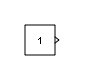
\includegraphics[width=0.2\textwidth]{fig/simulink/constant_block.png}
		\caption{常数模块图例}\label{fig:constant_block}
	\end{figure}
	%%%%%%%%%%%%%%%%%
	
	Constant 模块生成实数或复数常量值。在本次建模中,主要用于常值输入以及一些固定参数的表示。
	
	\item 将输入乘以常量 Gain
	
	%%%%%%%%%%%%%%%%%
	\begin{figure}[H]
		\centering
		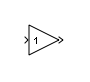
\includegraphics[width=0.2\textwidth]{fig/simulink/gain_block.png}
		\caption{增益模块图例}\label{fig:gain_block}
	\end{figure}
	%%%%%%%%%%%%%%%%%
	
	Gain 模块将输入乘以一个常量值(增益)。输入和增益可以是标量、向量或矩阵。在本次建模中,主要用于表示状态空间方程中,状态变量前面的系数。
	
	\item 输入信号的加减运算 Sum
	
	%%%%%%%%%%%%%%%%%
	\begin{figure}[H]
		\centering
		
\includegraphics[width=0.2\textwidth]{fig/simulink/sum_block.png}
		\caption{加减运算模块图例}\label{fig:sum_block}
	\end{figure}
	%%%%%%%%%%%%%%%%%
	
	Sum 模块对输入信号执行加减运算。Add、Subtract、Sum of Elements 和 Sum 模块是相同的模块。此模块可对标量、向量或矩阵输入执行加减运算。它还可以缩减信号的元素并执行求和。在本次建模中,主要用于表示状态空间方程中的加减运算。
	
	\item 可自定义函数模块 MATLAB Function
	
	%%%%%%%%%%%%%%%%%
	\begin{figure}[H]
		\centering
		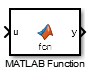
\includegraphics[width=0.2\textwidth]{fig/simulink/matlab_function_block.png}
		\caption{可自定义函数模块图例}\label{fig:matlab_function_block}
	\end{figure}
	%%%%%%%%%%%%%%%%%
	
	使用 MATLAB Function 模块可以编写用于 Simulink模型的 MATLAB函数。在本次建模中,主要用于表示较为复杂的判断与运算功能,给仿真带来一定便利。
	
	\item 饱和模块 Saturation
	
	将输入信号限制在饱和上界和下界值之间
	
	%%%%%%%%%%%%%%%%%
	\begin{figure}[H]
		\centering
		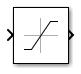
\includegraphics[width=0.2\textwidth]{fig/simulink/saturation_block.png}
		\caption{饱和模块图例}\label{fig:saturation_block}
	\end{figure}
	%%%%%%%%%%%%%%%%%
	
	Saturation 模块产生输出信号,该信号是在饱和上界和下界值之间的输入信号值。上界和下界由参数 Upper limit 和 Lower limit 指定。在本次建模中,主要用于限制相关变量的最大值,避免Inf无穷大值的发生而无法仿真。
	
	\item 显示输入常数值模块 Display
	
	%%%%%%%%%%%%%%%%%
	\begin{figure}[H]
		\centering
		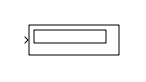
\includegraphics[width=0.2\textwidth]{fig/simulink/display_block.png}
		\caption{显示输入常数值模块图例}\label{fig:display_block}
	\end{figure}
	%%%%%%%%%%%%%%%%%
	
	Display 模块显示输入数据的值。您可以指定显示的格式和频率。在本次建模中,主要用于判断输入值是否合理,从而保证仿真的正常进行。
	
	\item 示波器 Scope
	
	%%%%%%%%%%%%%%%%%
	\begin{figure}[H]
		\centering
		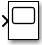
\includegraphics[width=0.1\textwidth]{fig/simulink/scope_block.png}
		\caption{示波器图例}\label{fig:scope_block}
	\end{figure}
	%%%%%%%%%%%%%%%%%
	
	Simulink Scope 模块显示时域信号。在本次建模中,主要用于输出随时间变化的状态变量,如速度,角速度等等。
	
	\item 合并变量模块 Mux
	
	将相同数据类型和数值类型的输入信号合并为虚拟向量
	
	%%%%%%%%%%%%%%%%%
	\begin{figure}[H]
		\centering
		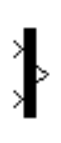
\includegraphics[width=0.1\textwidth]{fig/simulink/mux_block.png}
		\caption{合并变量模块图例}\label{fig:mux_block}
	\end{figure}
	%%%%%%%%%%%%%%%%%
	
	Mux 模块可将其输入合并为单个向量输出。输入可以是标量或向量信号。所有输入都必须具有相同的数据类型和数值类型。在本次建模中,主要用于合并输出结果,后续输出至工作空间。
	
	\item 写入工作区模块 To Workspace
		
	将相同数据类型和数值类型的输入信号合并为虚拟向量
	
	%%%%%%%%%%%%%%%%%
	\begin{figure}[H]
		\centering
		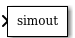
\includegraphics[width=0.2\textwidth]{fig/simulink/to_workspace_block.png}
		\caption{写入工作区模块图例}\label{fig:to_workspace_block}
	\end{figure}
	%%%%%%%%%%%%%%%%%
	
	To Workspace 模块将输入信号数据写入到工作区。在仿真期间,模块将数据写入到内部缓冲区。暂停仿真或仿真完成后,该数据将写入到工作区。在仿真暂停或停止之前,数据不可用。在本次建模中,主要将输出后结果,后续输出至工作空间进行处理作图。
	
	\item 创建模块封装 Subsystem mask
	
	为子系统和自定义模块创建自定义外观、创建用户定义的界面、封装逻辑以及隐藏数据。封装是用于模块的一种自定义用户界面。
	
	在对部分元件进行子系统封装后,可以进行Mask编辑:
	
	%%%%%%%%%%%%%%%%%
	\begin{figure}[H]
		\centering
		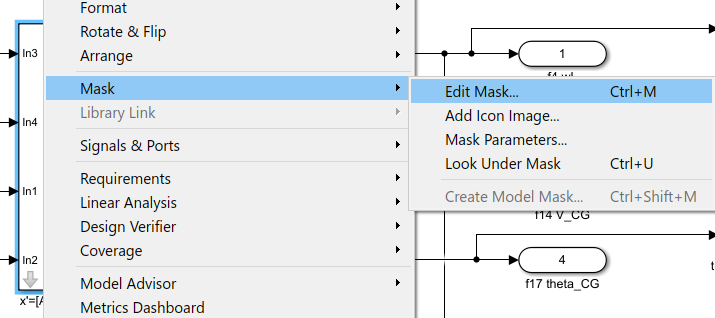
\includegraphics[width=0.85\textwidth]{fig/simulink/mask_operation.png}
		\caption{子系统封装操作图例}\label{fig:mask_operation}
	\end{figure}
	%%%%%%%%%%%%%%%%%
	
	在具体Mask界面中,可以直接添加相关参数编辑模块:
	
	%%%%%%%%%%%%%%%%%
	\begin{figure}[H]
		\centering
		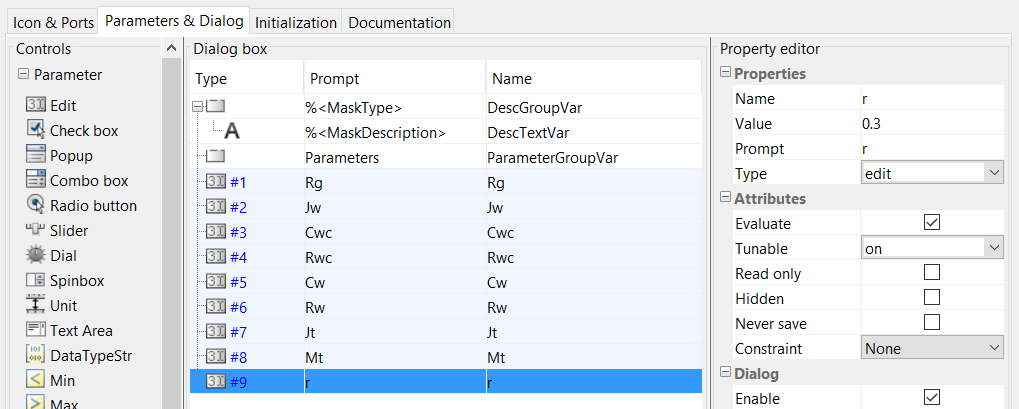
\includegraphics[width=0.85\textwidth]{fig/simulink/mask_interface.png}
		\caption{相关参数编辑操作图例}\label{fig:mask_interface}
	\end{figure}
	%%%%%%%%%%%%%%%%%
	
	在本次建模中,主要用于封装模型,以及快速参数调整。最终实现效果如下:
	
	%%%%%%%%%%%%%%%%%
	\begin{figure}[H]
		\centering
		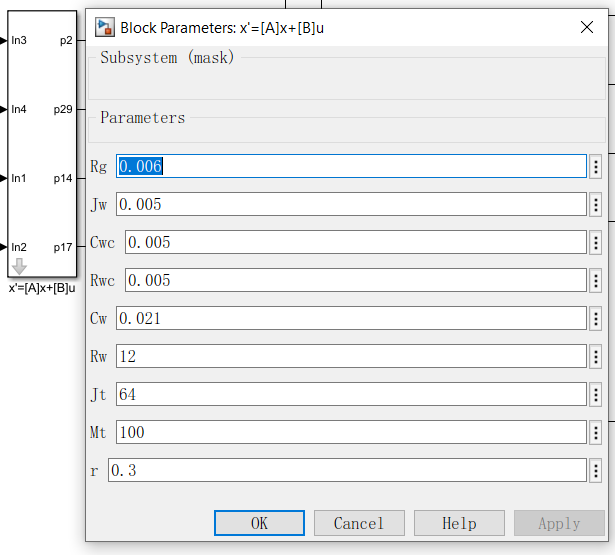
\includegraphics[width=0.85\textwidth]{fig/simulink/block_params.png}
		\caption{参数调整界面图例}\label{fig:block_params}
	\end{figure}
	%%%%%%%%%%%%%%%%%
	
	\subsection{系统框图仿真}
	\subsubsection{MPW 仿真}
	
	
	
	\subsubsection{MDM 仿真}
	
	
	\subsection{仿真条件详细说明} 
	
	我们采用 ode15s 解法器而不采用刚性系统常用的 ode113 解法器。 
	
	Ode113是一种变阶次多步 Adams-Bashforth-Moutlon 算法,此基于用前几个节点的值来计当 算法,此基于用前几个节点的值来计当 算法,此基于用前几个节点的值来计当 前节点的解,因此在相同精读下比 ode45和 ode23更快,比较适用于高阶或者需要大量计算的问题更快,比较适用于高阶或者需要大量计算的问题不适合于连续的系统。
	
	MATLAB推荐,ode45是大多数情况下的首选解法器。ode45 是基于 Dormand-Prince 4-5runge-kutta 公式,适用于一般非刚性系统的首选解法器。其精度较高,相比于其他解法器为中等水平。我们系统在 ode45解法器的仿真下,速度较慢且有时会出现无穷大溢出现象,故ode45解法器也无法满足我们的系统。
	
	而 ode15s 是基于数值微分公式 (NDF) 的变阶求解器。NDF 与后向差分公式(BDF,也称为 Gear 方法)有关,但比后者更高效。ode15s 求解器以数值方式生成 Jacobian 矩阵。
	在matlab建议下,如果怀疑某个问题是刚性问题,或者 ode45 失败或效率极其低下,请尝试 ode15s。经过测试,我们系统在 ode15s 解法器的仿真下,可以正常运行得到结果并且速度不慢故 ode15s 解法器可以满足我们的系统。
	
\end{itemize}
